\documentclass[a4paper]{article}

\usepackage[margin=1.5cm]{geometry}  % tweak margins as you like
\usepackage{graphicx}
\usepackage{subcaption}              % only for arranging panels (no sub-captions used)
\pagestyle{empty}
%\usepackage[numbers]{natbib}
%\usepackage[authoryear]{natbib}
\usepackage[numbers]{natbib}
%% The amssymb package provides various useful mathematical symbols
\usepackage{amssymb}
%% The amsmath package provides various useful equation environments.
\usepackage{amsmath}
\usepackage{epstopdf}
\usepackage{mathptmx,mathtools}
\usepackage{subcaption}
\usepackage{float} % Add this in your preamble
\usepackage[export]{adjustbox}
\usepackage{array} % Needed for m{} column type


\usepackage{amsmath}
\usepackage{nicefrac}
\usepackage{dirtytalk}
\usepackage{graphicx}   % For including images
\usepackage{tikz}       % For drawing arrows
\usepackage{xcolor}     % For coloring
\usepackage{lineno}
\renewcommand\linenumberfont{\normalfont\bfseries\small} % <-- Increase line number size

\begin{document}

\setcounter{figure}{5}

	\begin{figure}[!th] % Use [H] to prevent it from floating to the last page
	\centering
	% First subfigure
	\begin{subfigure}[t]{0.8\textwidth} % Use 80% of text width
		\centering
		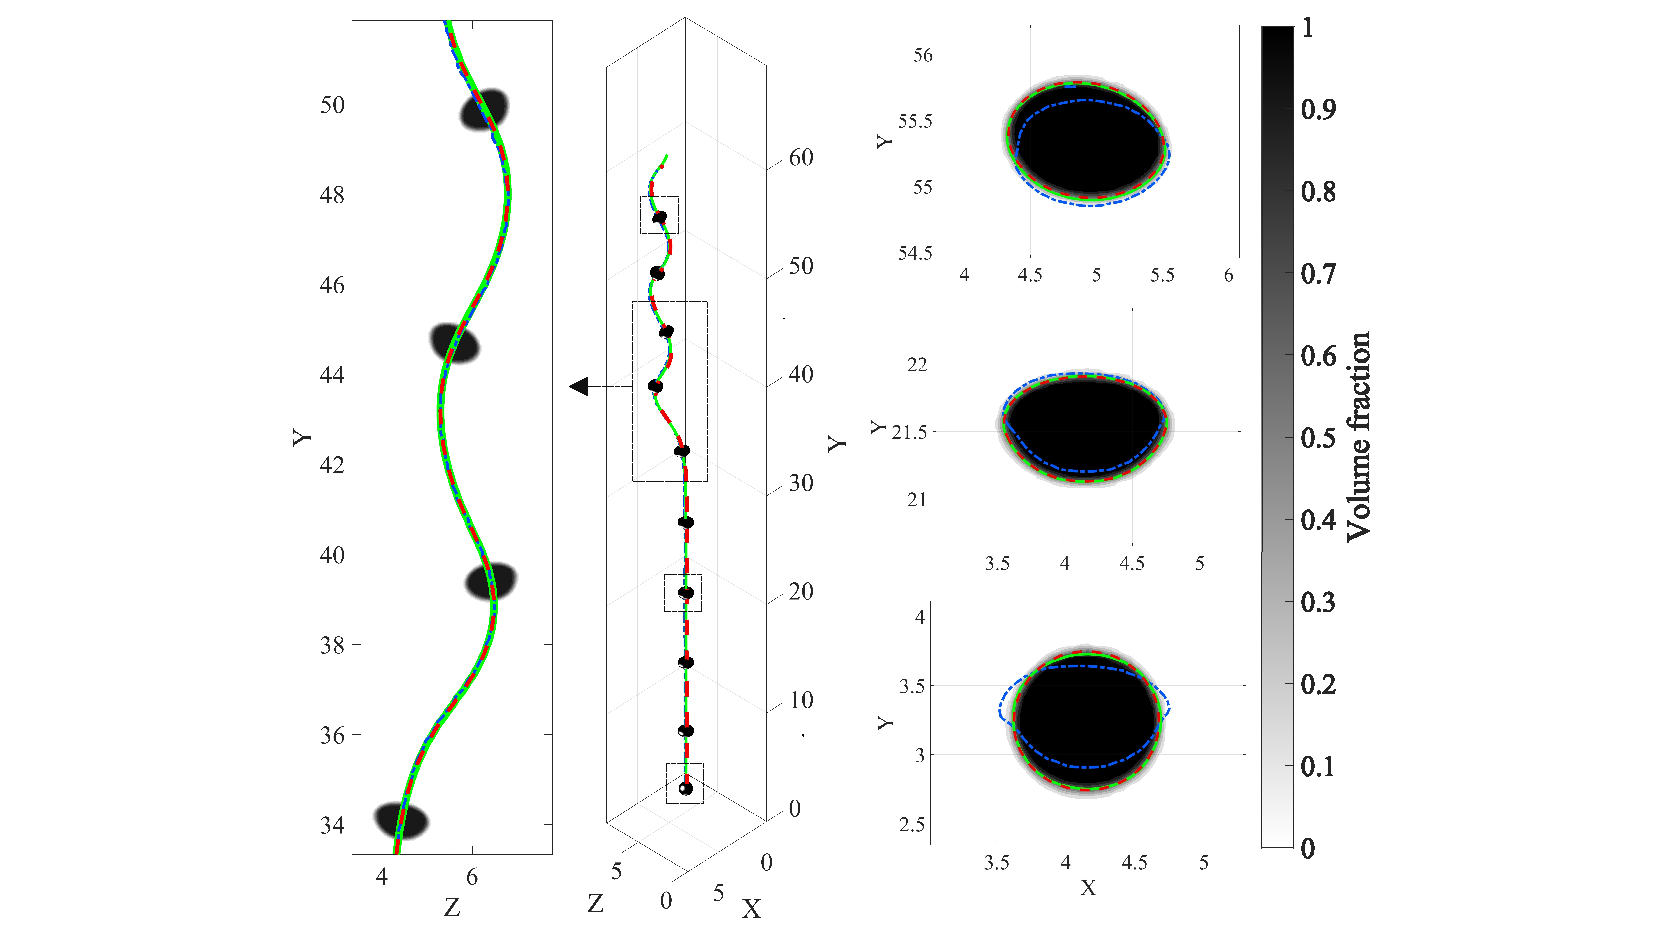
\includegraphics[scale=0.56,trim={4.5cm 0.0cm 4.5cm 0cm},clip]{Figure6a.pdf}
		\put(-120,236){\small\textbf{$\tau _{3} = 41.50$}}
		\put(-120,160){\small\textbf{$\tau _{2} = 14.01$}}
		\put(-120,80){\small\textbf{$\tau _{1} = 0.28$}}
		\put(-190,203){\small\textbf{$\tau _{3} $}}
		\put(-185,98){\small\textbf{$\tau _{2} $}}
		\put(-185,50){\small\textbf{$\tau _{1} $}}
		\put(-310,265){\textbf{(a)}}
		\vspace{0.3cm}
	\end{subfigure}
	
	% Second subfigure
	\begin{subfigure}[t]{0.8\textwidth} % Use 80% of text width
		\centering
		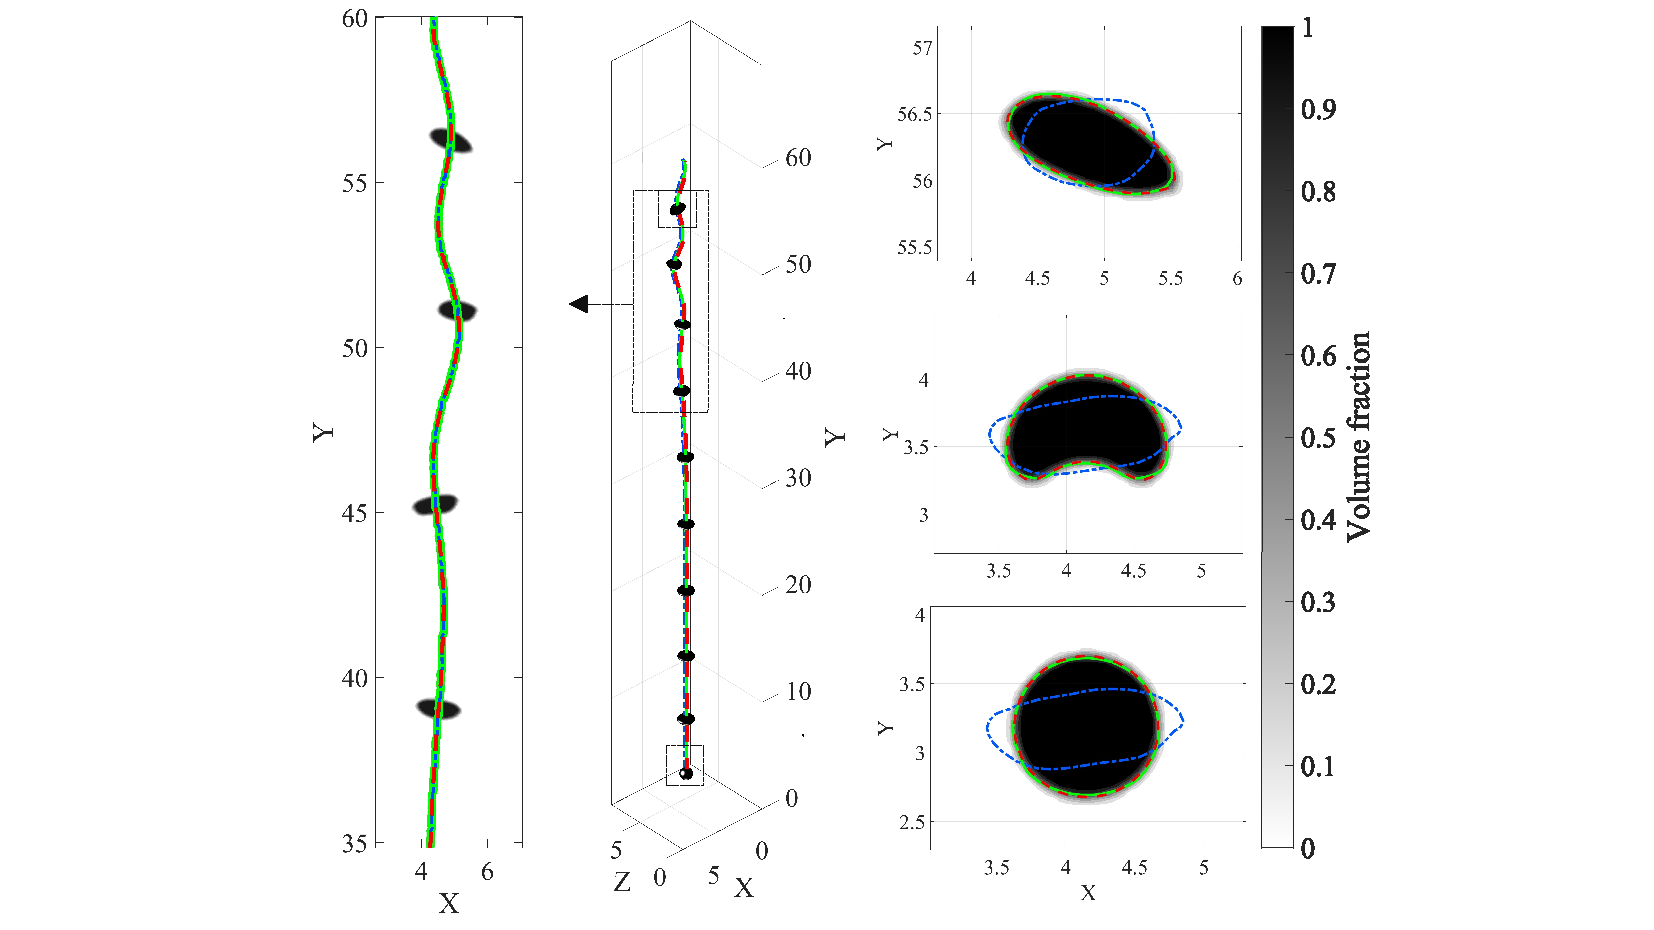
\includegraphics[scale=0.56,trim={4.5cm 0.0cm 4.5cm 0cm},clip]{Figure6b.pdf}
		\put(-120,236){\small\textbf{$\tau _{3} = 51.20$}}
		\put(-120,158){\small\textbf{$\tau _{2} = 0.76$}}
		\put(-120,79){\small\textbf{$\tau _{1} = 0.19$}}
		\put(-185,208){\small\textbf{$\tau _{3} $}}
		\put(-185,54){\small\textbf{$\tau _{1} $, $\tau _{2} $}}
		\put(-310,265){\textbf{(b)}}
	\end{subfigure}
	
	\caption{Rise trajectory and the 3D bubble interface at three intervals $\tau_{1}-\tau_{3}$ for cases (a) C$_4$ with 10 modes and (b) C$_5$ with 15 modes for interface and 10 modes for trajectory using ME-POD and ME-DMD schemes. The red dashed line, green solid line, and blue dash-dotted line denote the corresponding rise property obtained via DNS, ME-POD, and ME-DMD, respectively.}
	\label{Fig6}
\end{figure}

\end{document}